\chapter{Apprentissage profond}

  \section{Machine Learning}

    \subsection{Principes généraux}

      Le Machine Learning, également connu sous le terme d'apprentissage automatique, est un sous-domaine de l'intelligence artificielle, ayant vu le jour dans
      les années 1950\cite{Bib_Marr}\cite{Bib_McCar}
      Son champ d'application est aujourd'hui très vaste, et sa principale limite réside en la quantité d'informations exploitables, disponible au sein d'un domaine donné.

      L'accroissement de la collecte, du stockage et de la mise à disposition des données que nous connaissons depuis quelques années a permis l'essor de ces algorithmes et leur transposition à de nombreux problèmes :

      \begin{itemize}
	\item la classification de contenu audio-visuel au sens large, allant de l'image au sujet d'un texte ou d'une revue
	\item le filtrage de contenus, tels que les spams ou les intrusions sur les systèmes d'informations
	\item le tri et la sélection d'informations les plus pertinentes à délivrer via la publicité ou les flux de contenus des médias sociaux
	\item l'analyse et la prédiction de sentiments d'échantillons de population 
      \end{itemize}

      Plus précisément, ce concept recouvre les systèmes constitués de paramètres réglables, typiquement vus sous la forme de
      valeurs vectorielles, en vue de fournir la sortie attendue pour une série de valeurs données en entrée. En outre, ce type d'apprentissage se distingue
      par sa capacité à ajuster ses paramètres de manière autonome, en se basant sur l'expérience des données précédemment traitées.

      Dans ce qui va suivre, cette technique sera abordée à la lumière des problèmes de reconnaissance de formes, les entrées dont il sera alors question étant des images ou des vidéos.

    \subsection{Systèmes de reconnaissance de formes}

      L'architecture d'un système de reconnaissance de formes comprend deux éléments principaux :

      \begin{itemize}
	\item un extracteur des caractéristiques de l'entrée
	\item un classifieur qui donne le résultat en sortie, associant généralement l'entrée à une classe
      \end{itemize}

      Dans les années 50, les premiers modèles de reconnaissance étaient constitués d'un extracteur de caractéristiques "fait-main", peu modulaire et fastidieux à implémenter\cite{Bib_LeCun}.
      C'est lui qui est chargé de traduire l'image, ou partie de l'image, en une représentation vectorielle des motifs qu'elle contient.
      \par
      Dans un deuxième temps, le classifieur détermine la classe résultante selon une somme pondérée des composantes du \gls{carvec}.
      Une valeur seuil est fixée de telle sorte à ce que la sortie soit activée ou non en fonction du calcul précédent.
      Lorsque des erreurs sont repérées en sortie, cet algorithme va réajuster ses paramètres internes en vue d'améliorer les réponses suivantes. On parle alors d'entraînement.
      \par
      Dans le cadre d'une classification dite linéaire, ces réglages s'effectuent sur la valeur des poids associés aux caractéristiques.
      L'enjeu du classifieur est de réduire la différence entre les résultats attendus $\hat{y}$, et effectifs $y$.
      La phase d'entraînement revient à minimiser une fonction objectif\footnote{Dans le framework Caffe, une telle fonction est désignée sous le nom de loss function.}, en modulant les pondérations ($\theta$).
      D'un point de vue mathématique, la fonction objectif peut différer en fonction de l'approche adoptée. On la trouvera par exemple sous forme de moindres carrés de résidus\cite{Bib_WikiLS} :

      \begin{center} $ E = J({\theta}) =  \sum\limits_{i=1}^{n} (y_{i} - \hat{y}_{i} )^2 $ \end{center}

      ou d'erreur quadratique moyenne\cite{Bib_WikiMSE} :

      \begin{center} $ E = J({\theta}) =  \frac{1}{n}\sum\limits_{i=1}^{n} (y_{i} - \hat{y}_{i})^2 $ \end{center}

      Un tel comportement correspond à un apprentissage supervisé, où la réponse correcte est connue, permettant à la machine de s'améliorer. Une fois cette phase achevée, le système est théoriquement apte à
      classifier avec exactitude de nouvelles entrées, jusqu'alors inconnues : c'est la généralisation.
      \par
      D'autre part, comme représenté figure~\ref{fig:c1p1s2}, l'approche par apprentissage profond vise à étendre les capacités d'entraînement et de généralisation à l'ensemble de la chaîne de reconnaissance de formes.
      Notre étude se base sur ce dernier modèle, où l'extracteur de caractéristiques, aussi appelé noyau, peut être entraîné.

      \begin{figure}[H]
	  \centering
	  \makebox[\textwidth]{\includesvg[width=.6\paperwidth]{c1p1s2_schema}}
	  \caption{Différentes approches de la reconnaissance de formes}
	  \label{fig:c1p1s2}
      \end{figure}

  \section{Réseaux de neurones}

    \subsection{Neurone artificiel}

      A la base des réseaux de neurones se trouve le concept de neurone formel représenté sur la figure\ref{fig:c1p2s1}.
      \par
      \begin{figure}[H]
	  \centering
	  \makebox[\textwidth]{\includesvg[width=.4\paperwidth]{c1p2s1_neuron}}
	  \caption{Schéma d'un neurone formel}
	  \label{fig:c1p2s1}
      \end{figure}

      Nous retrouvons les entrées $x_{i}$ qui correspondent dans notre cas aux i composantes du vecteur de caractéristiques donné par l'extracteur.
      Ces entrées sont ensuite sommées avec leur poids $\theta_{i}$ (ou coefficient synaptique) respectif, ainsi qu'un coefficient $\theta_{0}$ appelé biais.
      Le résultat pondéré est ensuite transmis à une fonction d'activation non linéaire\cite{Bib_WikiAN}. Celle-ci activera la synapse suivante (ici, la sortie), si son résultat dépasse un seuil donné.
      \par
      En pratique, plusieurs fonctions d'activation peuvent être choisies au regard de leurs caractéristiques.
      Parmi les plus utilisées, on peut citer les fonctions sigmoïdes et tangentes hyperboliques. Leur efficacité tient notamment du fait qu'elles soient indéfiniement et rapidement dérivables et non polynômiales.
      \par
      Admettons que ce système contienne des entrées sous forme de vecteurs à $n$ dimensions, étiquettés selon les classes $C_{0}$ et $C_{1}$. Le but de l'entraînement sera d'obtenir en sortie : \\

      \begin{center}

      $\left\{
      \begin{array}{ll}
      y=0,$ si $ x\in C_{0} \\
      y=1,$ si $ x\in C_{1}
      \end{array}
      \right.\ , \forall x
      $

      \end{center}
      sachant que,
      \begin{center}
      $ y = \phi( \sum\limits_{i=1}^{n}(x_{i}\theta_{i}) + \theta_{0} ),$ avec $\phi$ fonction d'activation
      \end{center}

      le problème revient à trouver la valeur optimale du vecteur $\theta$, permettant de séparer linéairement les classes.
      La figure\ref{fig:c1p2s1_2} illustre ce concept dans le cadre d'une classification d'éléments à deux dimensions, distribués entre deux classes.

      \begin{figure}[H]
	  \centering
	  \makebox[\textwidth]{\includesvg[width=.4\paperwidth]{c1p2s1_points}}
	  \caption{Classes linéairement séparables}
	  \label{fig:c1p2s1_2}
      \end{figure}

    \subsection{Réseau multicouches}

      Les problèmes traditionnels de classification nécessitent des modèles plus élaborés, car ils sont souvent insolubles à l'aide de simples régressions linéaires. On dit que l'ensemble des éléments constituant nos classes
      sont non linéairement séparables (les résultats de la fonction XOR par exemple). On organise alors les neurones formels en successions de couches, ce qui permettra de diviser le plan en $n$ sous-ensembles, avec $n >2$.
      On appelle typiquement \textit{couche d'entrée} la première couche du réseau, \textit{couches cachées} les couches internes au réseau et \textit{couche de sortie} la dernière couche.
      Issue du site de tensorflow\cite{Bib_PlaygroundTF} (une librairie de calcul de machine learning développée par Google\cite{Bib_TenFlo}), la capture d'écran\ref{fig:c1p2s2} illustre les jeux de données pour lesquelles les régressions linéaires s'avèrent inefficaces.

      \begin{figure}[H]
	  \centering
	  \makebox[\textwidth]{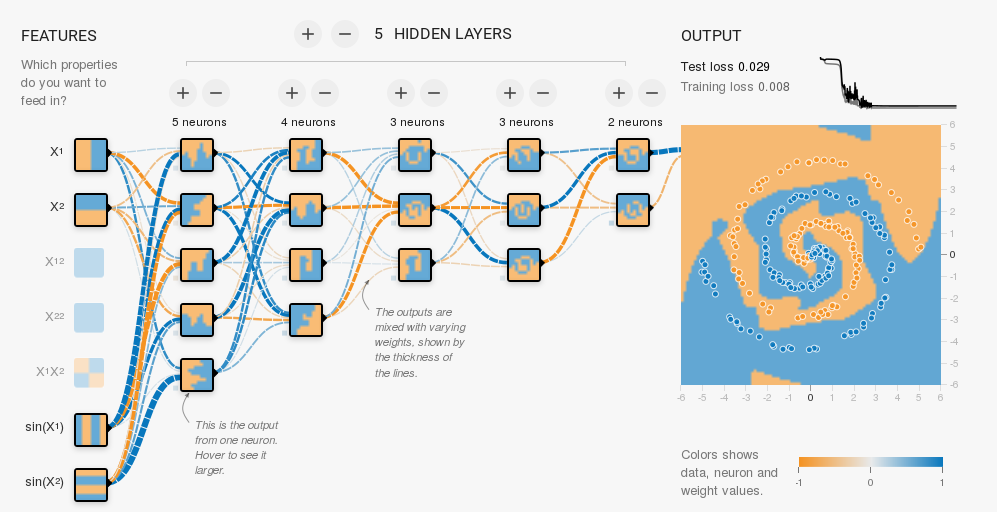
\includegraphics[width=.6\paperwidth]{c1p2s2_tensorflow}}
	  \caption{Simulation tensorflow}
	  \label{fig:c1p2s2}
      \end{figure}


      Dans cette configuration, les interactions entre les différents neurones, et les différentes couches, correspondent à ce qui a été décrit précédemment. L'information se propage `en avant` (\textit{forward propagation} ou \textit{feed forward}).
      \par
      Pour ajuster les poids synaptiques lors de l'entraînement, chaque neurone formel calcule l'erreur locale dûe à la modification d'un poids (c'est l'équivalent de l'erreur globale présentée section 1.1.2, limitée à deux neurones).
      La méthode de descente de gradient stochastique\cite{Bib_WikiSGD} va permettre d'estimer l'incrément ou le décrément d'erreur correspondant à la modification du poids en question. Cela consiste à dériver partiellement la fonction d'erreur par le poids local.

      \begin{center}
      $\Delta \theta_{i,j} = -\alpha \dfrac{\partial E} {\partial \theta_{i,j}} $ , avec
      $\left\{
      \begin{array}{ll}
      \Delta \theta_{i,j} $, variation de $\theta$ entre les neurones $i$ et $j$ $\\
      \alpha $, le pas d'apprentissage $\\
      E $, fonction d'erreur $
      \end{array}
      \right.
      $
      \end{center}

      Notons qu'une valeur de $\alpha$ élevée augmente le risque de dépasser le minimum recherché, tandis qu'une valeur trop petite va rallonger la phase d'entraînement.
      \par
      Les difficultés à calculer cette dérivée à n'importe quel niveau du réseau mènent à utiliser la technique de la rétropopagation\cite{Bib_WikiBP} (\textit{backpropagation}). L'erreur est alors estimée par la couche de sortie (qui a connaissance du résultat), puis relayée aux niveaux inférieurs, simplifiant ainsi leur descente de gradient respective.

  \section{Réseaux convolutifs}

    \subsection{Approche architecturale}

      L’approche adoptée par les \gls{CNN}s consiste en premier lieu à adapter la structure du réseau aux entrées reçues, à savoir des images.
      Les neurones sont organisés en 3 dimensions : hauteur, largeur et profondeur\footnote{Il faut bien faire la distinction entre la profondeur d’une couche, dont il est ici question, et celle du réseau en lui-même, qui signifie son nombre de couches}.
      Aussi, dans un tel réseau, les neurones seront seulement connectés à un nombre limité de neurones de la couche précédente.
      En définitive pour  $n$ classes, la sortie sera caractérisée par un vecteur résultant de dimensions $ 1 \times 1 \times n$.
      Une architecture de \gls{CNN} répandue est composée des couches suivantes. A titre d’exemple, nous avons choisi d’illustrer les dimensions des couches pour un système utilisant les entrées de la base \gls{CIFAR 10} RGB :

      \begin{itemize}
	\item \textbf{INPUT} : un volume 3D de [$32 \times 32 \times 3$]
	\item \textbf{CONV} : chaque neurone calcule le produit de convolution entre ses poids et une région locale connectée de la couche d’entrée. Le résultat se traduit comme un volume où la profondeur correspond au nombre de filtres utilisés (soit un volume en sortie de dimensions [$32 \times 32 \times 12$] si on utilise 12 filtres).

	\item \textbf{ReLU} (Rectified Linear Unit) : cette couche utilise pour chacun de ses neurones un rectificateur linéaire comme f(x) = max(x, 0). Une telle fonction élémentaire est appliquée sur chacune des composantes du volume précédent. La dimension de la sortie est invariante, soit dans notre exemple [$32 \times 32 \times 12$]. 
	\item \textbf{POOL} : sous-échantillonnage sur la hauteur et la largeur de la couche précédente. Le volume résultant sera par exemple dimensionné de la manière suivante : [$16 \times 16 \times 12$].
	\item \textbf{FC} (Fully Connected) : comme son nom l’indique, les unités de cette couche sont connectées à tous les neurones de la couche précédente. Le vecteur résultant est calculé en fonction de poids, de manière similaire aux \gls{MLNN}. La dimension en sortie sera [$1 \times 1 \times 10$].

      \end{itemize}
      Notons que l’entraînement d’un tel réseau, par descente de gradient, concerne les couches CONV et FC qui effectuent leurs calculs en fonction de poids et biais paramétrables. Les couches POOL et ReLU traitent leurs entrées de manière fixe, indépendamment de l’avancée de l’entraînement.

      \begin{figure}[H]
	  \centering
	  \makebox[\textwidth]{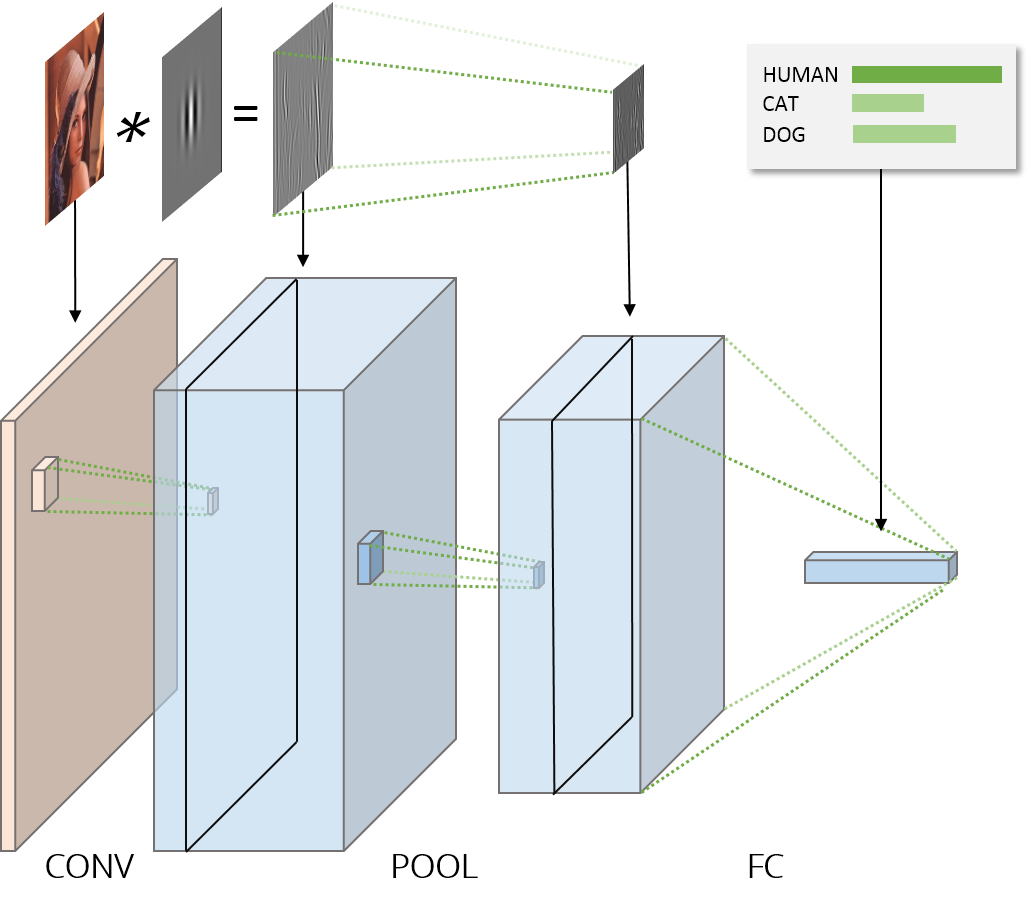
\includegraphics[width=.5\paperwidth]{c1p3s1}}
	  \caption{Evolution des données au sein d'un \gls{CNN} simple}
	  \label{fig:c1p3s1}
      \end{figure}

    \subsection{Convolution et pooling}
    
      Les paramètres des couches de convolution sont composés de filtres de même profondeur que la couche d’entée.
      Les largeurs et hauteurs sont quant à elles moindres, afin d’être appliquées à des zones réduites de l’image, constituant une fenêtre de traitement.
      Pour un filtre donné, les sous prélèvements locaux sont donc convolués avec les valeurs du filtre par glissement de la fenêtre dans une direction, jusqu’à ce que la surface entière ait été prise en compte.
      Le résultat de ces opérations se traduit en une « carte d’activation » à deux dimensions, traduisant la réponse d’une partie de l’image, puis de l’image entière, à la caractéristique contenue par le filtre.
      L’empilement des « cartes d’activation » des différents filtres vont constituer la profondeur de l’entrée de la couche suivante (ReLU).

      La disposition spatiale et le nombre de neurones présents dans le volume en sortie de la couche de convolution dépendent des 3 paramètres (aussi appelés hyper-paramètres) suivants :
      \par
      \begin{itemize}
	\item \textbf{La profondeur} du volume en sortie est donnée par le nombre de filtres utilisés. Est appelée « colonne de profondeur » (\textit{depth column}) un ensemble de neurones connectés à la même région de l’entrée.
	\item \textbf{$S$ : le pas} avec lequel on décale le filtre le long de l’entrée va également déterminer la dimension de la sortie. En effet, un grand pas entraînera une sortie réduite dans l’espace, tandis qu’un pas d’un pixel donnera une sortie de taille maximum.
	\item \textbf{$P$ : le padding à zéro}, qui consiste à compléter de part et d’autre le volume d’entrée avec des « $0$ ». L’intérêt de cette technique est de contrôler la taille du volume de sortie et, en particulier, de s’assurer qu’il soit égal à celui de l’entrée en hauteur et en largeur.
      \end{itemize}



      Etant données les variables suivantes :
      \begin{center}

      $\left\{
      \begin{array}{ll}
      W$ : taille de l’entrée (volume)$\\
      F$ : taille de la fenêtre de traitement de la couche de convolution$\\
      S$ : pas de glissement de la fenêtre de traitement$\\
      P$ : padding à zéro$
      \end{array}
      \right.
      $
      \end{center}

      le nombre de neurones nécessaires au volume de sortie est donné par :
      \begin{center}
      $ \dfrac{W-F+2P}{S}+1$
      \end{center}

      Notons que dans un réseau convolutif, le partage des paramètres permet de limiter leur quantité et la complexité des calculs qui en découlent.
      Cette technique s’appuie sur l’invariance d’une caractéristique, si on la translate dans l’espace.
      En effet, on s’aperçoit que des mêmes propriétés visuelles peuvent se trouver à différents endroits, dans une ou différentes images.
      Dans ce cas de figure, il devient pertinent d’utiliser les mêmes filtres (au sens de caractéristiques recherchées) sur l’ensemble de l’image d’entrée.
      De plus, un neurone s’occupant d’une partie de l’image, on partagera un filtre –pour une profondeur donnée– entre tous les neurones, de manière à respecter ce principe.
      Ainsi, on mutualise les paramètres et l’apprentissage qui en découle pour chacun des plans ($x_{i}$,$y_{i}$), avec $i  \in [0$ ; nombre de filtres$]$.
      Cette méthode montre ses limites lorsque la position d’une caractéristique recherchée est fixe pour tout un jeu de données d’entrée (apprentissage et généralisation).
      Par exemple, en considérant des chiffres toujours centrés sur l’image d’entrée, l’apprentissage effectué par les neurones responsables de cette partie de l’image ne sera d’aucune utilité pour les neurones traitant les coins.
      \par
      L’intérêt du pooling est de réduire progressivement la taille de la représentation de l’entrée ainsi que le nombre de paramètres et de calculs afférents.
      Cela s’effectue par la définition d’une fenêtre de traitement, puis la sélection de certaines unités pour chacune des zones de l’entrée.
      Le résultat consiste en un sous-échantillonnage de l’entrée qui, dans la pratique, s’appuiera sur des fonctions max ou moyenne sur les valeurs de la fenêtre.